\documentclass{beamer}
\usetheme{Madrid}
\usecolortheme{wolverine}

\usepackage{array}
\usepackage{xcolor}
\usepackage{tikz-cd}

\usepackage{user-commands}


%Information to be included in the title page:
\author{Nolan Pyott}
\institute{University of Waterloo}
\date{August 17, 2023}
\begin{document}

\title[Gen GCDs as Apps of Vojta's Conjecture]
{Generalized GCDs as Applications of Vojta's Conjecture}
\frame{\titlepage}

\begin{frame}{Setting the Stage}
    % Let's set the stage.
    % It's late, you have lots of work, and you're behind on most of it.
    % Naturally, you pull out a blank sheet of paper and start playing around with the sequence $2^n - 1$.
    
    
    % Completely discarding what you need to do,
    % you begin by writing down the factorization of some low power terms.

    Let's inspect $(2^n - 1)_{n \geq 1}$!

    \begin{align*}
        2^1 - 1 & = 1 \\
        2^2 - 1 & = 3 \\
        2^3 - 1 & = 7 \\
        2^4 - 1 & = 15 = 3 \times 5
    \end{align*}
\end{frame}

\begin{frame}{A Problem Emerges}
    % Clearly not always prime, 
    % you check out a similar sequence.

    What about another sequence?

    \begin{align*}
        3^1 - 1 & = 2 \\
        3^2 - 1 & = 8 = 2^3 \\
        3^3 - 1 & = 26 = 2 \times 13 \\
        3^4 - 1 & = 80 = 2^4 \times 5
    \end{align*}

    % While not quite always coprime,
    % the GCD between each term is always relatively small.

    There seems to be a pattern.
\end{frame}

\begin{frame}{Some Further Inspection}
    % You go as far to check this out for a variety of inputs $a^n  - 1$ and $b^n - 1$.
    % Even plotting down some of them with a computer.

    How about a log plot of the GCDs?

    \[
        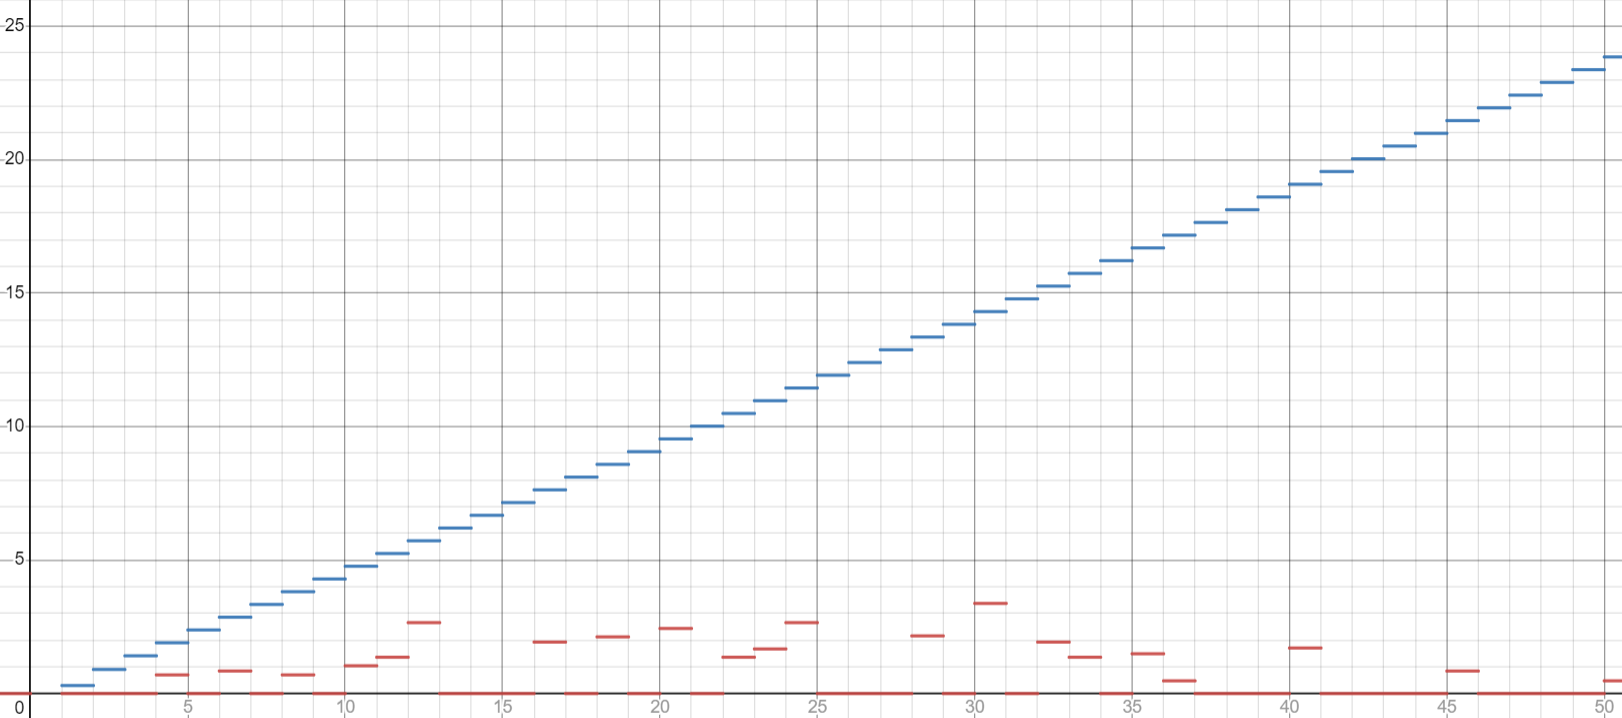
\includegraphics[scale=0.3]{presentation-images/plot-gcd-2n-3n.png}
    \]
\end{frame}

\begin{frame}{A Key Theorem}
    % Putting together everything you find,
    % you begin your sights on writing a conjecture and getting to work.
    % Before you can vindicate your time spent procrastinating more pertinent tasks,
    % you come across the following theorem.

    \begin{theorem}[Bugeaud, Corjava, Zannier 2002]
        Given two multiplicatively independent integers $a, b \in \Z$ at least $2$, and some $\varepsilon > 0$,
        we may eventually determine some $N \geq 1$ such that for $n \geq N$ thereafter
        \[
            \gcd(a^n - 1, b^n - 1) < \exp(\varepsilon n).
        \]
    \end{theorem}
\end{frame}

\begin{frame}{Where to?}
    % Naturally, if you're anything like myself,
    % you continue to ignore your other work and investigate this particular result.  
    % Specifically, you may want to know what actual tools were able to resolve this,
    % and where else could you go with the same tools and similar questions?

    \begin{itemize}
        \item How could you show this?
        \item Where does this generalize to?
        \item What did we \textit{really} stumble upon?
    \end{itemize}
\end{frame}

\begin{frame}{General Plan}
    % What we find, indeed, is that the tools used in the BCZ paper do have generalizations which apply to multiple different contexts.
    % Ultimately, the goal this morning will be to understand how the concept of the GCD can be generalized,
    % and how this generalization can be combined with a very deep conjecture of Paul Vojta to provide all sorts of conjectured generalizations of the BCZ result.

    \begin{itemize}
        \item Break down the key ideas from BCZ
        \item Generalize GCDs themselves
        \item Use Vojta's Conjecture to predict and affirm other results
    \end{itemize}
\end{frame}

\begin{frame}{Main Result on $\bbP^n$}
    \begin{theorem}
        Let $V \subset \bbP^n$ be a smooth variety of co-dimension $r \geq 2$ not intersecting any $\{x_i = 0\}$.
        Suppose as well that $V$ is given as the vanishing set of some $f_1, \ldots, f_m \in \Z[x_0, \ldots, x_n]$.
        
        Let $\varepsilon > 0$.
        Suppose that Vojta's conjecture is true.
        Then we may determine some $g \in \Z[x_0, \ldots, x_n]$ and $\delta$ only depending on $f_i$, 
        so that every coprime integer tuple $(a_0, \ldots, a_n) \in \Z^{n + 1}$ is either a root of $g$ or
        \begin{multline*}
            \gcd(f_1(a_0, \ldots, a_n), \ldots, f_k(a_0, \ldots, a_n)) \\
                \leq \max\{|a_0|, \ldots, |a_n|\}^\varepsilon
                    \cdot (|a_0 \cdots a_n|_S')^{\frac{1}{r - 1 + \delta \varepsilon}}.
        \end{multline*}
        
    \end{theorem}
\end{frame}

\begin{frame}{Main Result on Elliptic Curves}
    \begin{theorem}
        Let $C/ \Q$ be an elliptic curve.
        Assuming Vojta's conjecture,
        we then find that for any $\varepsilon > 0$ that there is a proper closed subvariety $Z \subseteq C^2$ such that for any points $P, Q \in C(\Q) \sm Z$,
        \[
            \gcd(D_P, D_Q) \leq (H(P) \cdot H(Q))^\varepsilon,
        \]
    \end{theorem}
\end{frame}

\begin{frame}{A Secret Ingredient}
    % Before we can get to these,
    % let's start off with our initial unconditional theorem.
    % While these exponentially growing sequences may be too sparse for some tool kits such as Sieve theory,
    % we may however turn to Diophantine Approximation.

    \begin{theorem}[Schmidt's Subspace Theorem]
        Take $L_1, \ldots, L_m: \Q^n \to \Q$ to be linearly independent set of linear forms.
        Fix some $\delta > 0$ and $C > 0$, 
        and consider the inequality
        \[
            \prod_{i = 1}^m |L_i(x_1, \ldots, x_n)|_v < (\max_{1 \leq j \leq n} |x_j|)^{m - n - \delta}.
        \]
        Then the coprime integer solutions $(x_1, \ldots, x_n) \in \Z^n$ lie in finitely many hyperplanes of $\Q^n$.
    \end{theorem}

    % Key idea of the above is that one or more of the linear forms is an approximation of some sort,
    % while the bound compares to an extent how much we're aasking from our integer coordinates with respect to their size.
\end{frame}

\begin{frame}{Initial Bound}
    Setup as
    \[
        \frac{c_n}{d_n} = \frac{b^n - 1}{a^n - 1},
        \qquad
        z_{n, j} = \frac{b^{nj} - 1}{a^n - 1}
    \]

    Cleverly using series expansion of $(a^n - 1)^{-1}$,
    for fixed $M > 1$
    \[
        \left|
            \frac{b^{jn} - 1}{a^n - 1}
            - \sum_{m = 1}^M \frac{b^{jn} - 1}{a^{mn}}
        \right|
        = \left|
            z_{n,j}
            - \sum_{m = 1}^M \frac{b^{jn}}{a^{mn}}
            + \sum_{m = 1}^M \frac{1}{a^{m n}}
        \right|
        \ll \frac{b^{jn}}{a^{n(M + 1)}}
    \]
\end{frame}

\begin{frame}{Failed Attempt}
    Fixing $J > 1$ and $N = J + M + MJ$,
    write coordinates
    \[
        \Q^N = \{
            (x_1, \ldots, x_N) = (
                z_1, \ldots, z_J, 
                u_1, \ldots, u_M,
                v_{1,1}, \ldots, v_{J,M}
            )\}.
    \]

    We use input vectors
    \[
        \vec{x}_n = d_n a^{Mn} (
            z_{n,1}, \ldots, z_{n,J},
            \tfrac{1}{a^n}, \ldots, \tfrac{1}{a^{Mn}},
            \tfrac{b^n}{a^n}, \ldots, \tfrac{b^{nJ}}{a^{Mn}}
        ),
    \]

    approximating linear forms $1 \leq j \leq J$
    \[
        L_{j, \infty}
        = z_j 
            + \sum_{m = 1}^M u_M
            - \sum_{m = 1}^M v_{j,m},
    \]
    and additional linear forms $J < j \leq N$
    \[
        L_{j, \infty} = x_i
    \]
\end{frame}

\begin{frame}{More Places to Compare}
    Let's add in the $p$-adic norms
    \[
        |p^k \tfrac{a}{b}|_p = p^{-k}.
    \]

    We call all norms $M_\Q$.

    \begin{itemize}
        \item Archimedean places $M_k^\infty$ is just usual absolute value $| \cdot | = |\cdot|_\infty$
        \item Non-archimedean places $M_\Q^0$ are $p$-adic norms $| \cdot |_p$
    \end{itemize}
\end{frame}

\begin{frame}{Extending Schmidt's Theorem}
    Extension by Ridout

    \begin{theorem}
        Let $S \subseteq M_\Q$ be a finite set of places, fix $1 \leq n \leq m$.
        Take $L_{1,v}, \ldots, L_{m, v} : \Q^n \to \Q$ to be linearly independent set of linear forms.
        Fixing $\delta > 0$ and $C > 0$
        \[
            \prod_{v \in S}\prod_{i = 1}^m |L_{i,v}(x_1, \ldots, x_n)|_v < (\max_{1 \leq i \leq n} |x_i|)^{m - n - \delta}.
        \]
        Then the integer solutions $(x_1, \ldots, x_n) \in \Z^n$ with $\gcd(x_1, \ldots, x_n) = 1$ to the above lie in finitely many hyperplanes of $\Q^n$.
    \end{theorem}

\end{frame}

\begin{frame}{More Places, More Results}
    Remaining ingredients: 
    \begin{itemize}
        \item Use $S^0 \subseteq M_\Q^0$ all dividing $ab$, and $S = S^0 \cup \{ \infty \}$. 
        \item Add linear forms $L_{i, v} = x_i$, balances out bound in product
        \item Throw in contradictory assumption for $\gcd(a^n - 1, b^n - 1)$,
            make choices for $M$ and $J$,
            obtain desired bound for Subspace Theorem
        \item Too many integers, not enough hyperplanes, derive contradiction
    \end{itemize}
\end{frame}

\begin{frame}{Arithmetic Complexity}
    % With generalization in mind,
    % we need to reformulate in terms of the language of Diophantine approximation.
    
    Consider from Diophantine approximation:

    \begin{theorem}[Roth's Theorem]
        Given an algebraic number $\alpha \in \R$, for any $\varepsilon > 0$,
        there exists at most finitely many co-prime integers $p, q \in \Z$ such that
        \[
            \left|\alpha - \frac{p}{q}\right| < \frac{1}{|q|^{2 + \varepsilon}}.
        \]
    \end{theorem}

    % Considering the inequality from Roth's Theorem,
    % we consider how good the approximation is relative to how much arithmetic complexity is required.
    % We may write the height as

    Complexity captured by \textit{height} as

    \[
        H(p/q) = \max(|p|, |q|).
    \]
\end{frame}

\begin{frame}{Projective Height Functions}
    Account for multiplication by common factor with $p$-adic absolute values.

    For $(x_0 : \cdots : x_n) \in \bbP^n(\Q)$,
    \[
        H(x_0 : \cdots : x_n)
        = \prod_{v \in M_\Q} \max_{0 \leq j \leq n} |x_j|_v
    \]
\end{frame}

\begin{frame}{Extending our Norms}
    For $k/\Q$, we have similar idea.

    By embedding $\sigma : k \hookrightarrow \C$, we obtain archimedean norms
    \[
        \|x\|_\sigma = |x|^{[k_\sigma : \R]}.
    \]

    For a prime ideal $\Fp$ of ring of integers $R_k$,
    \[
        \|x\|_\Fp = N_{k/\Q}(\Fp)^{-\ord_\Fp(x)}.
    \]

    All places for field denote $M_k$,
    with $M_k^\infty$ for archimedean and $M_k^0$ for non-archimedean.
\end{frame}

\begin{frame}{Heights on Algebraic Integers}
    If we know $k/\Q$,
    \[
        H_k(x_0 : \cdots : x_n) = 
            \prod_{v \in M_k} \max_{0 \leq j \leq n} \|x_j\|_v
    \]

    Well-defined \textit{absolute height} as $H(P) = H_k(P)^{1/[k : \Q]}$.
    Commonly use $h(P) = \log H(P)$ for \textit{logarithmic height}.
\end{frame}

\begin{frame}{Extending Height Functions}
    If we have a space $X$ and a map $\varphi : X \to \bbP^n$,
    we obtain
    \[
        h_\phi(P) = h(\phi(P))
    \]

    \begin{itemize}
        \item Which spaces can we use?
        \item Which maps make sense?
    \end{itemize}
\end{frame}

\begin{frame}{Schemes}
    Ring $R$ prime ideals $\Spec(R)$.
    This is an \textit{affine scheme}.

    \begin{itemize}
        \item Closed sets
        \[
            V(I) = \{ P \in \Spec(R) : I \subseteq P \}
        \]
        \item Open basis
        \[
            D_f = \{ P \in \Spec(R) : f \notin P \}
        \]
        \item Functions given by ring elements,
        restrictions by localization 
    \end{itemize}

    \begin{definition}
    A \textit{scheme} $X$ is a topological space with a \textit{sheaf} of functions $\cO_X$,
    locally isomorphic to an affine scheme.
    \end{definition}
\end{frame}

\begin{frame}{Basic Spaces}
    Use $\A^n_k = \Spec(k[x_1, \ldots, x_n])$.
    Note the maximal ideals are points,
    prime ideals irreducible algebraic subsets.

    Also have $\bbP^n_k = \Proj(k[x_0, \ldots, x_n])$, built with homogeneous ideals,
    notation using $V_+(I)$ and $D_+(f)$.
    
    Locally,
    \[
        D_+(x_i) = \Spec(k[\tfrac{x_j}{x_i}]) \cong \A^n,
    \]
    idea is to specialize to $x_i = 1$ in terms of coordinates.
\end{frame}

\begin{frame}{Weil Divisors}
    Spaces need an origin! We can get close.
    
    A \textit{Weil Divisor} is a formal sum of co-dimension one closed subschemes.
    Principal divisors as
    \[
        \rmDiv(f) = \sum_{\codim(Y, X) = 1} v_Y(f) Y.
    \]

    $\Div(X)$ is group under addition, principal divisors subgroup. 
    Quotient $\Cl(X)$ is \textit{Class Group}.

    Under some nice assumptions, equivalent to \textit{Cartier Divisors},
    \[
        D = \{ (U_i, f_i) \}_{i \in I}.
    \]

    Generally equivalent to \textit{invertible sheaves}, like $\cO(n)$.
\end{frame}

\begin{frame}{The Canonical Divisor Class}
    Given $A$-algebra, can construct \textit{module of relative differentials} $\Omega_{B/A}$.
    Glue together to give sheaf $\Omega_{X/Y}$.

    \begin{example}
    For $\bbP^1$ with coordinates $(x : y)$, we have $\Omega_{\bbP^1 / k}$ generated by $d(x/y)$ on $D_+(y)$ and $d(y/x)$ on $D_+(x)$.
    Thus
        \[
            \Omega_{\bbP^1 / k } \cong \cO(-2)
        \]
    \end{example}

    $\Omega_{X/k}$ has full rank when $X$ is smooth. 
    Thus we write $\omega_X = \wedge^n \Omega_{X / k}$.
    
    In particular
    \[
        \omega_{\bbP^n} \cong \cO(-n - 1).
    \]
\end{frame}

\begin{frame}{Maps Associated to Divisors}
    Consider sub-module of $K(X)$ given by
    \[
        L(D) = \{ f \in K(X) : D + \rmDiv(f) \geq 0 \}.
    \]
    Vector space when $k \subseteq \cO_X(X)$, so basis
    \[
        L(D) = \Span_k \{ f_0, \ldots, f_n \}.
    \]
    Hence, consider $\varphi : X \to \bbP^n$
    \[
        \varphi(P) = (f_0(P) : \cdots : f_n(P)).
    \]
\end{frame}

\begin{frame}{Weil's Height Machine}
    Association $D \mapsto h_D$ such that
    \begin{itemize}
        \item Unique up to $O(1)$, equivalent under linear equivalence
        \item Matches our original projective heights
        \item $h_{\varphi^* D} = h_D \circ \varphi$
        \item $h_{D_1 + D_2} = h_{D_1} + h_{D_2} + O(1)$
    \end{itemize}

    Geometric properties now become arithmetic properties!
\end{frame}

\begin{frame}{Local Height Functions}
    Can consider heights related to distance functions.
    \[
        \lambda_{D, v}(P) = - \log |f(P)|_v + O_v(1)
    \]

    Local height functions combine with \textit{local to global principal} for Weil's height machine
    \[
        h_D(P) = \frac{1}{[k : \Q]} \sum_{v \in M_k} \lambda_{D, v}(P) + O(1).
    \]

    For $H = \{ F(x) = 0 \} \subseteq \bbP^n$,
    \[
        \lambda_{H,v}(P) = \max_{0 \leq j \leq n} \log \left| \frac{x_j^d}{F(P)} \right|_v.
    \]
\end{frame}

\begin{frame}{Revisiting the GCD}
    Write $v^+(x) = \max(0, - \log |x|_v)$,
    find
    \[
        \log \gcd (a, b) = \sum_{v \in M_\Q} \min \{ v^+(a), v^+(b) \}.
    \]
    For origin $H = (0 : 1) \in \bbP^1$ $\bbP^1$,
    \[
        \lambda_{H,v}(a : 1) = v^+(a)
    \]
    GCD \textit{should} be local height for $(0, 0) \in \bbP^1 \times \bbP^1$.
\end{frame}

\begin{frame}{Blow ups of Varieties}
    For $Y \subseteq X$, we have $\pi : \wt X \to X$ and universal property
    \[
        \begin{tikzcd}[ampersand replacement=\&]
            Z \arrow[r, hook] \arrow[ddr] \arrow[drr, dashed] \& W \arrow[ddr] \arrow[drr, dashed] \& \\
            \& \& E \arrow[r, hook] \arrow[dl] \& \wt X \arrow[dl] \\
            \& Y \arrow[r, hook] \& X \&
        \end{tikzcd}
    \]
    \begin{itemize}
        \item Can be computed locally
        \item Birational map where we now have codim 1 subscheme $E$
        \item Separates ``lines" passing through $Y$ 
    \end{itemize}
\end{frame}

\begin{frame}{Computing Local Heights on Blow ups}
    \begin{lemma}
        Let $X/k$ be a non-singular variety and $Y \subseteq X$ of codim $\geq 2$.
        If $Y$ is given as the intersection of effective divisors $\{D_i\}_{i = 1}^m$,
        then the local Weil height for any $P \in X \sm Y$ with respect to the divisor $E$ and place $v \in M_k$ is given by
        \[
            \lambda_{E, v}(\pi^{-1}(P)) = \min\{\lambda_{D_i, v}(P)\}_{i = 1}^m.
        \]
    \end{lemma}
\end{frame}

\begin{frame}{The Generalized GCD}
    \begin{definition}[Generalized GCD]
        Suppose $X/k$ is a smooth variety, with a closed subvariety $Y$ of co-dimension at least 2.
        Let $\pi : \wt X \to X$ be the blowup of $X$ along $Y$, 
        and take $E = \pi^{-1}(Y)$ to be the exceptional divisor.
        We may then define the \textit{generalized logarithmic greatest common divisor} for a point $P \in (X \sm Y)(k)$ as
        \[
            h_{\gcd}(P; Y) = h_{\wt X, E}(\pi^{-1}(P)).
        \]
    \end{definition}
\end{frame}

\begin{frame}{Some Examples}
    Simplifying notation on $\bbP^1$, 
    for $X = \bbP^1 \times \bbP^1$ and $Y = (0, 0) \in X$,
    \[
        h_{\gcd}((a, b); Y) = \log \gcd (a, b).
    \]
    For $Y = V(f_1, \ldots, f_m) \subseteq \bbP^n$,
    \[
        h_{\gcd}(P; Y) = \log \gcd( f_1(P), \ldots, f_m(P)) + O(1).
    \]
\end{frame}

\begin{frame}{Vojta's Conjecture}
    Write \textit{proximity function} $m_S(D, P)$ and \textit{counting function} $N_S(D, P)$ as
    \[
        m_s(D, P)
        = \sum_{v \in S} \lambda_{D, v}(P), 
        \qquad
        N_S(D, P) = \sum_{v \notin S} \lambda_{D, v}(P).
    \]

    \begin{alertblock}{Vojta's Conjecture}
        Let $X/k$ be a non-singular projective variety and $k$ a number field.
        Take $A$ to be a big divisor, 
        $D$ a normal crossings divisor,
        and $K$ the canonical divisor class on $X$.
        Then for any $\varepsilon > 0$,
        there exists a proper closed subset $Z$,
        depending on all choices made,
        such that for any $P \notin Z$
        \[
            m_S(D, P) + h_{K}(P) \leq \varepsilon h_A(P) + O(1).
        \]
    \end{alertblock}
\end{frame}

\begin{frame}{A Conditional Result}
    Let $X/k$ be smooth with $Y \subseteq X$ a smooth subvariety of codim $r \geq 2$.
    Let $A$ be ample,
    and $-K_X$ is a normal crossings such that $\supp(-K_X) \cap Y = \emptyset$.

    \vspace{5mm}

    Assuming Vojta's conjecture,
    for finite $S \subseteq M_k$ finite,  and $0 < \varepsilon < r - 1$,
    there is a closed subvariety $Z \subsetneq X$ and a constant $\delta \in \R$,
    with $\delta$ only depending only on $X$, $Y$, and $A$,
    such that for any $P \in (X \sm Z)(k)$
    \[
        h_{\gcd}(P; Y)
            \leq \varepsilon h_{A}(P) + \frac{1}{r - 1 + \delta \varepsilon} N_S(-K_X, P) + O(1).
    \]
\end{frame}

\begin{frame}{Setting up Proof}
    Let $\pi : \wt X \to X$ be the blow up w.r.t $Y$ and $\pi^{-1}(Y) = E$.

    \vspace{5mm}
    
    Up to linear equivalence
    \[
        K_{\wt X} = \pi^* K_X + (r - 1)E.
    \]

    \vspace{5mm}
    
    As $A$ is ample, we write
    \[
        \pi^*A = \wt A + m E.
    \]

    \vspace{5mm}

    From $\supp(K_X) \cap Y = \emptyset$,
     $-\pi^* K_X$ is normal crossings.

\end{frame}

\begin{frame}{Applying Vojta's Conjecture}
    Taking $\varepsilon > 0$, $S \subseteq M_k$, $\wt P = \pi^{-1}(P)$,
    \begin{align*}
        & m_S(-\pi^*K_X, \wt P)
        + h_{K_{\wt X}}(\wt P)
        \leq \varepsilon h_{\wt A}(\wt P)
        + O(1) \\ \\
        \Rightarrow
        & -m_S(K_X, \pi(\wt P))
        + h_{K_X}(\pi(\wt P))
        + (r - 1)h_{E}(\wt P) \\
        & \leq \varepsilon h_{A}(\pi(\wt P))
            - \varepsilon m h_{E}(\wt P)
            + O(1)
    \end{align*}
    
    \vspace{5mm}
    
    Recalling generalized GCD,
    \[
        N_S(K_X, P)
        + (r - 1)h_{\gcd}(P; Y)
        \leq \varepsilon h_A(P)
        - \varepsilon m
        h_{\gcd}(P; Y) + O(1).
    \]

    \vspace{5mm}
    
    Further arrangement and setting $\delta = m$,
    \[
        h_{\gcd}(P; Y)
        \leq \varepsilon h_A(P)
        + \frac{1}{r - 1 + \delta \varepsilon} N_S(K_X, P)+ O(1).
    \]
\end{frame}

\begin{frame}{Our Main Result on $\bbP^n$}
    Using logarithms, want
    \begin{multline*}
        \log \gcd (f_1(P), \ldots, f_m(P)) \\
        \leq \varepsilon \log \max(|a_0|, \ldots, |a_n|)
        + \frac{1}{r - 1 + \delta \varepsilon} \log |a_0 \cdots a_n|'_S.
    \end{multline*}
    Apply main result with $X = \bbP^n$, $Y = V(f_1, \ldots, f_n)$, $A = \{ x_0 = 0 \}$.
    \begin{itemize}
        \item $h_{\gcd}(P; Y) = \log \gcd (f_1(P), \ldots, f_m(P)) + O(1)$
        \item $h_A(P) = \log \max(|a_0|, \ldots, |a_n|)$
        \item $N_{S \cup \{ \infty \}}(-K_{\bbP^n}, P)
        = -\log \prod_{p \notin S} |a_0 \cdots a_n|_p = \log |a_0 \cdots a_n |_S'$
    \end{itemize}
    Put together, and apply exponential function.
\end{frame}

\begin{frame}{Elliptic Curves}
    \textit{Elliptic curve} given by Weierstrass equation with $4A^3 + 27B^2 \neq 0$
    \[
        C = \{ y^2z = x^3 + Axz^2 + Bz^3 \} \subseteq \bbP^2.
    \]
    \begin{itemize}
        \item Canonical class is trivial. 
        \item Fixing identity point $O = (0 : 1 : 0)$, sub-group $\langle P - O \rangle \subseteq \Pic^0(C)$. Can use lines and Bézout's Theorem.
        \item Can write $P = (x_P, y_P)  \in C(\Q)$ as 
        \[
            x_P = \frac{A_P}{D_P^2}, \qquad y_P = \frac{B_P}{E_P^3}.
        \]
    \end{itemize}
    
\end{frame}

\begin{frame}{GCDs on Elliptic Curves}
    Let $Y = (O, O) \in C \times C$.
    Compute with $\rmDiv(z/x) = 2O$ that for $v \in M_\Q^0$
    \[
        \lambda_{O, v}(P) = \frac{1}{2} v^+(x_P^{-1}) = -\log |D_P|_v.
    \]
    Taking $p_1, p_2 : C \times C \to C$,
    \begin{align*}
        h_{\gcd}((P, Q); (O, O))
        & = \sum_{v \in M_\Q} \min (\lambda_{p_1^* O, v}(P, Q), \lambda_{p_2^* O, v}(P, Q)) \\
        & = \sum_{v \in M_\Q^0} \min(- \log |D_P|_v, -\log |D_Q|_v) \\
        & = \log \gcd (D_P, D_Q).
    \end{align*}
\end{frame}

\begin{frame}{Our Main Result on Elliptic Curves}
    Set $X = C \times C$, $Y = (O, O)$, and $A = p_1^* O + p_2^* O$, and apply main theorem with $K_C = 0$.
    \begin{itemize}
        \item $h_{\gcd}((P, Q); Y) = \log \gcd (D_P, D_Q)$
        \item $h_A((P, Q)) = h_O(P) + h_O(Q) = h(P) + h(Q)$
        \item For any $S \subseteq M_\Q$, $N_S(-K_C, (P, Q)) = 0$
    \end{itemize}
\end{frame}

\begin{frame}{A Special Case of Vojta's Conjecture}
    \begin{theorem}
        Let $C/k$ be a smooth elliptic curve where the group $C(\Q)$ is rank one.
        Suppose a birational $k$-morphism $f : X \to C \times C$,
        where $X$ is a non-singular, projective $k$-scheme.
        Moreover, suppose that the image of the exceptional set is contained in a finite subset of $(C \times C)(k)$.
        If $L$ is a big divisor on $X$,
        $D$ is the zero divisor with trivial height function,
        and $K_X$ is the canonical divisor,
        then for any $\varepsilon > 0$,
        there exists an effectively computable proper closed subset $Z \subseteq X$ for which $P \in (X \sm Z)(k)$ implies that
        \[
            h_K(P) \leq \varepsilon h_L(P) + O(1).
        \]
    \end{theorem}
\end{frame}

\begin{frame}{Conclusion}
    \begin{itemize}
        \item Do divisibility sequences return to small GCDs?
        \item Can unconditional versions be shown?
        \item Are any of the results able to be converted to effectively computable?
    \end{itemize}
\end{frame}

\begin{frame}
    Thanks to my peers, faculty, and professors over my time here at the Unversity of Waterloo.
    Special thanks to the audience here today,
    my readers Professors Jason Bell and Matt Satriano, 
    and especially my supervisor Professor David McKinnon.

    \vspace{5mm}

    Any additional questions?
\end{frame}

\end{document}
